\documentclass[conference]{IEEEtran}

\usepackage{graphicx}
\usepackage{float}
\usepackage{afterpage}
\usepackage{hyperref}
\usepackage{listings}
\usepackage{import}
\usepackage{algorithm2e}
\usepackage{tabularx}
%\usepackage{caption}

%bib
\bibliographystyle{IEEEtran}

% correct bad hyphenation here
\hyphenation{op-tical net-works semi-conduc-tor}

% path to figures
\graphicspath{{figures/}}

% for CFG listing
%\DeclareCaptionFormat{myformat}{#1#2#3}
%\captionsetup{format=myformat}
%\captionsetup[lstlisting]{position=bottom,belowskip=10pt}

\begin{document}
%
% paper title
% can use linebreaks \\ within to get better formatting as desired
\title{6p-Web Application Model Generation \\through Reverse Engineering and UI Pattern Inferring}

% author names and affiliations
% use a multiple column layout for up to three different
% affiliations
\author{
\IEEEauthorblockN{Clara Sacramento}
\IEEEauthorblockA{Department of Informatics Engineering,\\ Faculty of Engineering of the \\University of Porto \\Porto, Portugal \\ei09090@fe.up.pt}
\and
\IEEEauthorblockN{Ana C. R. Paiva}
\IEEEauthorblockA{INESC TEC, Department of Informatics Engineering, \\Faculty of Engineering of the \\University of Porto \\ Porto, Portugal \\apaiva@fe.up.pt}}


% use for special paper notices
%\IEEEspecialpapernotice{(Invited Paper)}

%ACP -------

% É preciso clarificar que não há contribuições na execução dos testes.
% tem que se fazer uma discussão dos resultados comparativos das duas diferentes abordagens
% dizer explicitamente qual é a research question %%%check
% ver o trabalho do Artemis (Mesbah)
% corrigir o abstract no que diz respeito aos modelos introduzirem bugs %%%check
% corrigir a informação do algoritmo 1
% Mudar o nome da subsecção para File Processing (LogProcessor) %%%check
% reformatar listing 1 %%%check
% explicar o que é o epsilon %%%check
% colocar refs de model/metamodel inference e de DSLs 

%--------

% make the title area
\maketitle

\begin{abstract}
A great deal of effort in model-based testing is related to the creation of the model. The model itself, while a powerful tool of abstraction, can have conceptual errors, introduced by the tester. This paper presents a dynamic reverse engineering approach that aims to extract part of the model of an existing Web application through the identification of User Interface (UI) patterns. This approach explores any Web application via reverse engineering, records information related to the interaction (interaction history, HTML pages and their URLs), analyzes the gathered information, and infers the UI patterns via a set of heuristics rules. After complemented with additional information, the model extracted is the input for the Pattern-Based GUI Testing (PBGT) approach for testing existing applications.
\end{abstract}
\begin{IEEEkeywords} Reverse Engineering, Web Application, UI Patterns, Web Scraping \end{IEEEkeywords}

\IEEEpeerreviewmaketitle

\section{Introduction}\label{sec:intro}

Web applications are getting more and more important, and can now handle tasks that before could only be performed by desktop applications \cite{garrett2005ajax}, like editing images or creating spreadsheet documents. However, despite their growing relevance, they still suffer from a lack of standards and conventions \cite{constantine2002usage}, unlike desktop and mobile applications. This means that the same task can be implemented in many different ways, which makes automated Web application testing difficult to accomplish and inhibits reuse of testing code. For instance, authentication (\textit{login}) failure usually triggers the appearance of an error message, but some implementations simply erase the inserted data, with no error message visible.

% por exemplo o login válido pode implicar uma mudança de página ou uma mensagem de erro ou simplesmente apagar a informação introduzida e continuar na mesma página
%%% check

Graphical User Interfaces of all kinds are populated with recurring behaviors that vary slightly, an example being authentication (\textit{login/password}) and content search. These behaviors (patterns) are called User Interface (UI) patterns \cite{van2001patterns} and are recurring solutions that solve common design problems. Due to their widespread use, UI patterns allow users a sense of familiarity and comfort when using applications. 

However, while UI patterns are familiar to users, their implementation may vary significantly.  Despite this, it is possible to define generic and reusable test strategies (User Interface Test Patterns - UITP) to test those patterns. This requires a configuration process, in order to adapt the tests to different applications \cite{morgado2012gui}. 

That is the main idea behind the PBGT (\textit{Pattern-based GUI Testing}) project, in which this research work is included. In the PBGT approach, the user builds a test model of the Web application with instantiations of UI Test Patterns, and later uses that model to test the Web app. The model can be built manually by the user, but this is a morose process and not recommended, since it may introduce conceptual errors. Half the bugs found through model-based testing are conceptual errors in the model itself and not bugs in the system to test \cite{dalal1999model}.

The goal of the work described in this paper is to continue the work done in \cite{nabuco2013inferring} on the reverse engineering process (PARADIGM-RE), whose aim is to automatize the model construction: independently/automatically explore a Web application, infer the existing UI patterns in its pages, and finally produce a model with the UI Test Patterns that define the strategies to test the UI Patterns present in the web application. This speeds up model construction, and hopefully introduces less errors into the model.

The rest of the paper is structured as follows. Section \ref{sec:pbgt} presents an overview of the PBGT project, setting the context for this work.  Section \ref{sec:re} describes the developed approach, its components and  their interrelations, and the results it produces. Section \ref{sec:eval} provides a practical example of the proposed system. Section \ref{sec:sota} addresses the related work, as well as the available tools to perform the needed tasks. Section \ref{sec:conc} presents the conclusions, some of the problems encountered and a perspective on future work. 

\section{PBGT Overview}\label{sec:pbgt}

As mentioned before, the focus of this paper is a component of a research project named PBGT (\textit{Pattern-based GUI Testing}) \cite{moreira2013pattern}. The goal of this project is to develop a model-based GUI testing tool and approach, usable as an industrial tool.

\subsection{Architecture}
This project has five parts: a DSL (\textit{Domain Specific Language}) named \textbf{PARADIGM} to define GUI testing models based on UI Test Patterns; \textbf{PARADIGM-RE}, a Web application reverse engineering tool whose purpose is to extract UI patterns from Web pages without access to their source code, and use that information to generate a test model written in PARADIGM; a modeling and testing environment, named \textbf{PARADIGM-ME}, built to support the creation of test models; an automatic test case generation tool, named \textbf{PARADIGM-TG}, that generates test cases from test models defined in PARADIGM; and finally, a test case execution tool, named \textbf{PARADIGM-TE}, which executes test cases, analyzes their coverage, and returns detailed execution reports. The architecture and workflow of the project is shown in Fig. \ref{fig:pbgt}.

\begin{figure}[!htb]
\centering
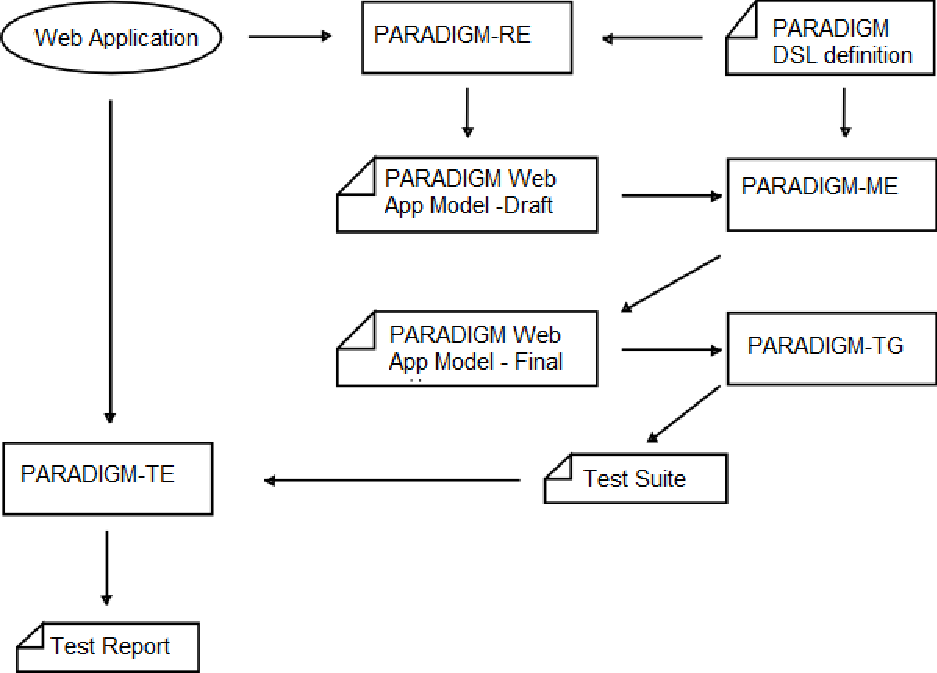
\includegraphics[width=0.45\textwidth]{pbgt}
\caption{An overview of the PBGT project}
\label{fig:pbgt}
\end{figure}

\subsection{PARADIGM DSL}
%falar doc conetores e, do init e do end, e falar também dos elementos estruturais: Form e Group

The definition of the PARADIGM DSL has started by analyzing a set of existing UI Patterns \cite{van2001patterns}. This DSL contains a set of UI Test Patterns that specify generic test strategies to test those UI Patterns along their different implementations. Besides UI Test Patterns, the DSL also defines a set of connectors that allows the definition of sequences of test strategies to execute.

A UI Test Pattern defines a test strategy which is formally defined by a set of test goals (for later configuration) \cite{moreira2013pattern} with the form:

\begin{equation}< Goal; V; A; C; P >\end{equation}\label{eq:ui}

\textit{Goal} is the ID of the test. \textit{V} is a set of pairs { [\textit{variable}, \textit{inputData}] } relating test input data with the variables involved in the test. \textit{A} is the sequence of actions to perform during test case execution. \textit{C} is the set of possible checks to perform during test case execution, for example, “check if it remains in the same page”. \textit{P} is a Boolean expression (precondition) defining the set of states in which it is possible to execute the test.

The UI Patterns defined in the PARADIGM language are:
\begin{itemize}
\item[] \textbf{Login}: This pattern is commonly found in Web applications, especially in the ones that restrict access to functionalities or data. Usually consists of two input fields (a normal input box for email or username, and a cyphered text for the password) and a submit button, with optionally a ``remember me'' checkbox. The authentication process has two possible outcomes: valid and invalid.
\item[] \textbf{Search}: This pattern consists of one or more input fields, where the user inserts keywords to search, and a submit button to start the search. The search may be submitted via a submit button, or dynamically upon text insertion. When the search is successful, the website shows a list of results; upon failure, an error message may be shown.
\item[] \textbf{Sort}: This pattern sorts a list of data by a common attribute (price, name, relevance, etc.) according to a defined criteria (ascending or descending, alphabetically, etc.).
\item[] \textbf{Master Detail}: This pattern is present in a webpage when selecting an element from a set (called \textit{master}) results in filtering/updating another related set (called \textit{detail}) accordingly. For example, clicking on a checkbox associated to a brand may include (or exclude) products of that brand in a product search result list. Generally the only elements changed are the elements belonging to the \textit{detail} set.
\item[] \textbf{Menu}: This pattern is very common in webpages. It's usually defined as a tree structure with several navigational options, to provide easier access for users. 
\item[] \textbf{Input}: This pattern is any kind of input field that allows the user to insert text.
\item[] \textbf{Call}: This pattern is any kind of element where a click triggers a change of page.
\end{itemize}

\subsection{Produced Models}

The models produced by the reverse engineering tool PARADIGM-RE consist of a XML file that contains information about the UI Test Patterns needed to test the UI Patterns found: their name and the input values for their variables. The PARADIGM model generated by the PARADIGM-RE tool does not contain the connectors between the UI Test Patterns, the checks to perform during test case execution, or the pre-condition determining the states where the test strategy will be run. This information needs to be complemented by the tester afterwards in order to generate test cases and execute them over a web application.

\section{Reverse Engineering Approach}\label{sec:re}

\subsection{Previous Work}\label{sec:pw}

The  approach described in this paper aims to improve on the previous work \cite{nabuco2013inferring} done on the PARADIGM-RE tool. The previous tool extracted information from an user's interaction with the Web application under analysis, analysed the information, produced some metrics (such as the total ratio of the LOC (\textit{lines of code}), length of all visited pages and the ratio of two subsequent pages), and finally used those metrics and the user interaction's information to infer UI patterns via a set of heuristic rules. \\
The information saved from a user interaction is the source code and URLs of the visited pages, and the interaction's execution trace. An execution trace is the sequence of user actions executed during the interaction with a software system, such as clicks, text inputs and also some information of the system state (e.g., the information that is being displayed). An example of an execution trace file used by the tool can be seen in Table \ref{tab:exec}.

\begin{table}[!htb]
\resizebox{0.5\textwidth}{!}{
  \begin{tabular}{| c | c | c |}
     \hline
     \textbf{Action} & \textbf{Target} & \textbf{Value} \\ \hline
     type&id=input\_username &``user1" \\ \hline
     type&id=input\_password &``123pass" \\ \hline
     clickAndWait & css=input[type=``submit"]&EMPTY \\
     \hline
     type&id=searchInput&``coffee" \\ \hline
	 clickAndWait & id=mw-searchButton&EMPTY\\
     \hline
     select&id=sort&label=Price:Low to High \\
     \hline
  	 \end{tabular}
}
\caption{Example of an execution trace file.}
\label{tab:exec}
\end{table}

The approach identified almost all of the available patterns (excepting \textit{Menu }and \textit{Call}), but produced a high number of false positives \cite{nabuco2013inferring}, and the exploration process was done enirely by the user interaction with the Web application under test. \\

The work described in this paper has the same primary aim as the previous tool (to identify UI patterns in the Application Under Test (AUT)), but has other goals. The first is to remove the need for user interaction with the AUT to identify patterns, by providing a reverse engineering process to explore automatically the web application under analysis. The second is to refine and improve the pattern inferring process, and lower or eliminate completely the percentage of false positives. The third is to identify more patterns than the previous tool.\\

The architecture of the tool is seen in Figure \ref{fig:retool}.

\begin{figure}[!htb]
\centering
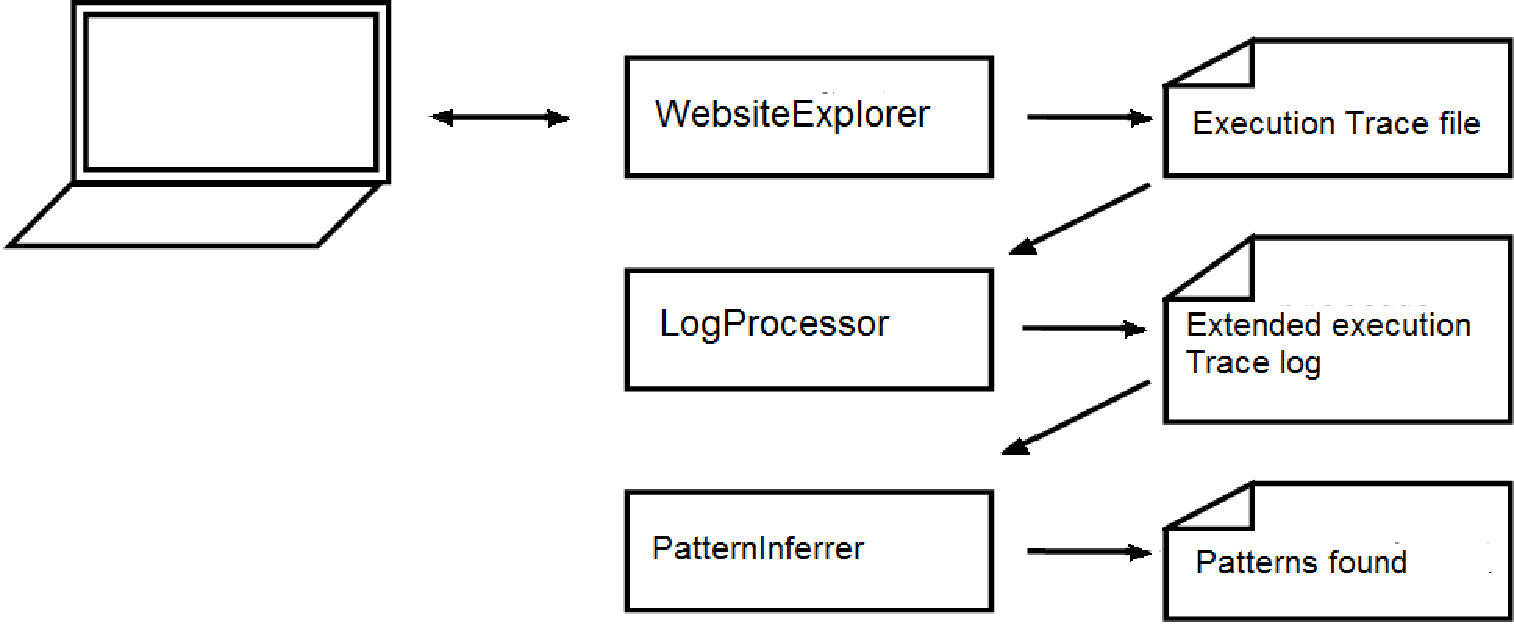
\includegraphics[width=0.45\textwidth]{retool}
\caption{The architecture of the approach.}
\label{fig:retool}
\end{figure}

The approach can be divided into three parts: \textbf{WebsiteExplorer}, \textbf{LogProcessor}, and \textbf{PatternInferrer}.

\textbf{WebsiteExplorer} interacts automatically with the AUT and produces an execution trace file with the actions taken (see Table \ref{tab:exec} for an example). \textbf{LogProcessor} is a text parser. It analyzes the previous file, parses each line, searches for important keywords and uses them to identify the action contained in the line, and produces an updated execution trace file (see Table \ref{tab:exec1} for an example). Finally, \textbf{PatternInferrer} analyzes the updated execution file, identifies the existent patterns, their location in the website and any existing parameters, and produces an XML file with the results.

\subsection{AUT Exploration (WebsiteExplorer)}\label{sec:inter}
The interaction process is described in a simplified manner in Algorithm \ref{alg:seeker}.

\begin{algorithm}
  %\SetLine
  \KwData{number\_of\_actions, number\_of\_iterations, website\_base\_url, configuration\_file}
  \KwResult{execution\_trace\_file}
  
  current\_action := 0; redirections := 0\;
  configuration := parseConfigurationFile()\;
  
  \While{current\_action $<$ configuration.number\_of\_actions}{
    \If{configurations.isSearchingForMenu()}
      {
        menuElements.add(getMenuElementsInPage())\;
      }
    \If{configuration.isSearchingForMasterDetail()}
    {
      masterElements.add(getMasterElementsInPage())\;
      detailElements.add(getDetailElementsInPage())\;
    }
  
  	list := extractValidNonVisitedElements\;
    next\_element := chooseNextElement(list)\;
  \eIf{next\_element == null}
  {%then
  	redirections++\;
    \eIf{redirection $<$ configuration.number\_of\_iterations}
    	{%then
        	go\_to\_base\_URL\;
            write\_to\_execution\_trace\_file\;
        }
        {%else
        	end\_program\;
        }
  }
  {%else
  	visit(element)\;
    visitedElements.add(element)\;
    write\_to\_execution\_trace\_file\;
    current\_action++;
  }
  wait(configuration.politenessDelay)\;
}

\caption{Pseudo-code algorithm to explore a page.}\label{alg:seeker}
\end{algorithm}

Currently the elements explored are \textit{$<$select$>$} elements, \textit{$<$input$>$} elements, and \textit{$<$a$>$} (link) elements. The way each element is visited is different: link elements are clicked; input elements get text (either a keyword or a number, depending on the type of input) and the containing form is submitted; and in the case of dropdown menus, a random option is selected and the surrounding form is submitted. The exception to the \textit{input} rule is when the element is identified as a \textit{login} element, in which case all the sibling elements (elements inside the form where the selected element is located) get text and only then the form is submitted.

Information about these elements is extracted via XPath\footnote{XPath: \url{www.w3schools.com/XPath/}}. Before interacting with an element, the algorithm makes the following checks: if the element has not been visited in the current page, and finally, if the element contains any unwelcome keywords that if explored may drive the explorer into unwanted ways. These keywords may be general to all elements (anything that edits information or contains the words 'buy'/'sell', for example, that would lead to purchase products) or element-specific (input elements cannot contain the attribute '\textit{disabled}' or'\textit{readonly}', if they are to be interacted with). All elements have the same probability of being chosen from a list of elements.

The execution trace file produced is a CSV (\textit{Comma-separated values}) file with three columns: \textbf{action}, the type of action executed (\textit{click, type}, or \textit{select} when selecting an option in a dropdown menu -- it may also contain the suffix \textit{AndWait}, which indicates a page change); \textbf{target}, the identifier of the visited element; and \textbf{value}, which has the parameter for the action and may be empty (for example, in the case of \textit{type} actions, it is the inserted text).

The exceptions are the Menu and MasterDetail patterns. Since the explorer can't be relied on to explore every element belonging to these patterns in each page, elements belonging to these patterns are found through analysing the current page source and extracting all elements that obey a set of rules. These are passed directly to the \textbf{PatternInferrer} to be written in the final output file (see Section \ref{sec:inf}).

\subsection{Action File Processing (LogProcessor)}\label{sec:fp}

This component is a lexical analyzer, whose role is to examine the execution trace file line by line and identify the type of each action written therein. It has a data structure (which serves as its lexical grammar) containing the rules it is going to search for, and each has the following attributes: \textbf{pattern\_name}, the identifier for the rule; \textbf{identifying\_regex}, a regex (Regular Expression\footnote{Regex: \url{http://www.regular-expressions.info/}}) that identifies an action of that type; and \textbf{garbage\_removal\_regex}, another regular expression that serves to erase unneeded words in case the pattern is discovered. 

For every line, all rules are tested, and if a rule matches the line, first a camel-case token (composed by the sum of the action type and the rule's name) is produced; and afterwards all words that match the \textit{garbage\_removal\_regex} are removed. This is done because a pattern may be a superclass of another pattern, and in that case it is better to just identify the super pattern. For example, if an element is identified as part of a \textit{search} pattern, it is not necessary to identify it as \textit{input} as well.

The identifiable patterns by default are: \textit{login, search, sort}, and \textit{input}. However, the identifiable patterns can also be overridden and added to via a text file.

An example of file processing may be seen in Table \ref{tab:exec}.

\begin{table}[!htb]
\resizebox{0.5\textwidth}{!}{
  \begin{tabular}{| c | c | c || c |}
     \hline
     \textbf{Action} & \textbf{Target} & \textbf{Value} & \textbf{Processing Return} \\ \hline
     type&id=input\_username &``user1"&typeUsername \\ \hline
     type&id=input\_password &``123pass"&typePassword \\ \hline
     clickAndWait & css=input&EMPTY&clickFormSubmit \\
      & [type=``submit"] & & PageChange\\
     \hline
     type&id=searchInput&``coffee"&typeSearch \\ \hline
	 clickAndWait & id=mw-searchButton&EMPTY&clickSearch\\
      & & & PageChange \\ \hline
     select&id=sort&label=Price: &selectSort \\
      & & Low to High& \\
     \hline
  	 \end{tabular}
}
\caption{Example of an execution trace file, and of processed lines.}
\label{tab:exec1}
\end{table}

\subsection{UI Pattern Inferring (PatternInferrer)}\label{sec:inf}
This component is a syntactical analyzer, that takes as input the extended execution trace file returned by the LogProcessor, runs it against a predefined grammar, and returns the patterns found. If during the process the tool detects the same UI Pattern instance several times, the tool is capable of ignoring it. Its reasoning is explained in Figure \ref{fig:inferrer}.

\begin{figure}[!htb]
\centering
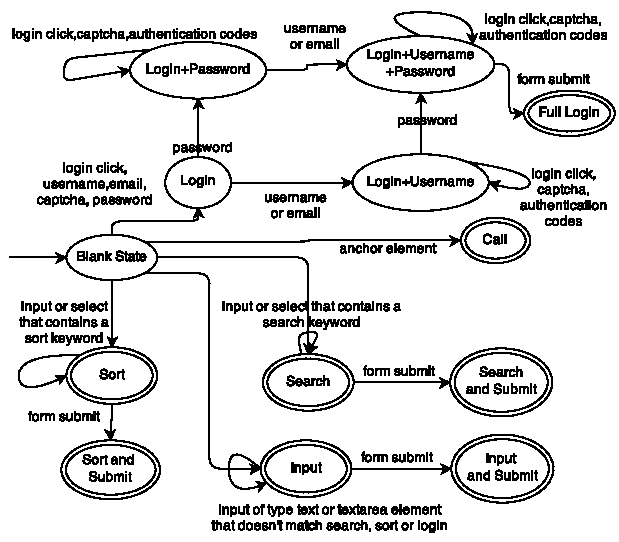
\includegraphics[width=0.45\textwidth]{Global_State_Machine.pdf}
\caption{The inferrer's reasoning algorithm, expressed in a finite state machine.}
\label{fig:inferrer}
\end{figure}

For simplicity's sake, only the valid paths are shown in the figure. All patterns except Login can be valid even in the absence of a form submit action; this is done to account for dynamic submission. In the case of the Login pattern, there can only be one password and one username or email record; this is done to distinguish login forms from register forms and password/email change forms.

After the file is processed, an XMI file is produced containing all the pattern occurrences found, and the values assigned to each variable, as per Equation \ref{eq:ui}. As mentioned before, the checks to be done on each variable and any preconditions must be specified by the tester later on in the PARADIGM-ME tool.

\section{Evaluation}\label{sec:eval}

\subsection{Research Questions}
\begin{itemize}
  \item[R1)] Is it possible to infer UI Test Patterns from a Web application without relying on user interaction?\\
  \item[R2)] Is it possible to improve the results provided by the previous tool?\\
\end{itemize}
\subsection{Evaluation Results}

The RE tool was initially experimented iteratively over a training set of Web applications, with the goal of refining and fine-tuning the strategies used to find UI Patterns.

After the training phase, the RE tool was used to detect UI Patterns in several public known and widely used Web applications, in an evaluation set. This time, the purpose was to evaluate the RE tool, i.e., determine which UI pattern occurrences the tool was able to detect in each application execution trace (ET) and compare them to the patterns that really exist in such trace. To verify if the results obtained from this tool are better than the results produced by the previous tool, all paths run through a Web application were run through both reverse engineering applications.

Five applications were chosen from the top 30 most popular Websites\footnote{according to: \url{en.wikipedia.org/wiki/List_of_most_popular_websites‎}}: Amazon, Wikipedia, Ebay, Youtube and Yahoo.

The results are presented in a table that shows the number of instances of each UI pattern that exist in the ET, the ones that the tools correctly found and the ones that the tools mistakenly found (false positives). The numerical results were combined and can be found in Table \ref{tab:eval}.

\begin{table}[!htb]
\resizebox{0.5\textwidth}{!}{
  \begin{tabular}{| c | c | c | c | c |}
     \hline \multicolumn{5}{|c|}{\textbf{Previous Tool}} \\ \hline
     \textbf{Pattern} & \textbf{Present} & \textbf{True} & \textbf{False} & \textbf{False} \\
       & \textbf{in ET} & \textbf{Positive} & \textbf{Negative} & \textbf{Positive} \\ \hline
     Login & 2 & 2 & 0 & 0\\
     Search & 14 & 11 & 3 & 0\\
     Sort & 2 & 1 & 1 & 0\\
     Input & 6 & 4 & 2 & 0\\
     MasterDetail & 61 & 58 & 3 & 0\\
     \hline
     \textbf{Total} & \textbf{85 (100\%)} & \textbf{76 (89\%)} & \textbf{9 (11\%)} & \textbf{0} \\ \hline 
     \hline \multicolumn{5}{|c|}{\textbf{Current Tool}} \\ \hline
     \textbf{Pattern} & \textbf{Present} & \textbf{True} & \textbf{False} & \textbf{False} \\
       & \textbf{in ET} & \textbf{Positive} & \textbf{Negative} & \textbf{Positive} \\ \hline
     Login & 2 & 2 & 0 & 0\\
     Search & 14 & 11 & 3 & 0\\
     Sort & 2 & 1 & 1 & 0\\
     Input & 6 & 4 & 2 & 0\\
     Call & 61 & 58 & 3 & 0\\ 
     Menu & 61 & 58 & 3 & 0\\
     MasterDetail & 61 & 58 & 3 & 0\\ \hline
     \textbf{Total} & \textbf{85 (100\%)} & \textbf{76 (89\%)} & \textbf{9 (11\%)} & \textbf{0} \\
     \hline
  	 \end{tabular}
}
\caption{Evaluation set results.}
\label{tab:eval}
\end{table}

As we can see in Table \ref{tab:eval}, during the case study the tool found no false positives, and found 89\% of the  patterns present in the ET. However, the case study does not mention how many patterns were present in the web applications that weren't visited, which we have not verified. Only one path produced by the application was considered for each Web application.

\section{Related Work}\label{sec:sota}

Reverse engineering is ``the process of analyzing the subject system to identify the system components and interrelationships and to create representations of the system in another form or at a higher level of abstraction'' \cite{chikofsky1990reverse}. There are four methods of applying reverse engineering to a system: the dynamic method, in which the data is retrieved from the system at run time without access to the source code, the static method, which obtains the data from the system source code \cite{systa1999dynamic}, the hybrid method, which combines the two previous methods, and the historical method, which extracts information about the evolution of the system
from version control systems, like SVN\footnote{SVN: svn.apache.org} or GIT\footnote{GIT: git-scm.com} \cite{canfora2011achievements}. These approaches follow the same main steps: collect the data, analyze it and represent it in a legible way, and in the process allow the discovery of information about the system's control and data flow \cite{pacione2003comparative}.

There are plenty of approaches that extract information from Web applications \cite{sampath2007applying,amalfitano2010rich, andjelkovic2011trace}. ReGUI \cite{coimbra2011reverse,coimbra2012dynamic} is a dynamic reverse engineering tool made to reduce the effort of modeling the structure and behavior of a software application GUI. It was also developed to reduce the effort of obtaining models of the structure and behaviour of a software
application's GUI, however it only works in desktop applications.
%%% 
Duarte, Kramer and Uchitel defined an approach for behavior model extraction which combines static and dynamic information \cite{duarte2006model}.

There are also plenty of approaches that explore Web applications for analysis and processing. Ricca and Tonella's ReWeb \cite{ricca2001understanding} dynamically extracts information from a Web application's server logs to analyze its structure and evolution, and so aims to find inconsistencies and connectivity problems. Benedikt \textit{et al.} introduced a framework called VeriWeb \cite{benedikt2002veriWeb} that discovers and explores automatically Web-site execution paths that can be followed by a user in a Web application. Bernardi \textit{et al.} \cite{bernardi2008reverse} presents an approach for the semi-automatic recovery of user-centered conceptual models from existing web applications, where the models represents the application's contents, their organization and associations, from a user-centered perspective. Marchetto \textit{et al.} proposed a state-based Web testing approach \cite{marchetto2008state} that abstracts the Document Object Model (DOM) into a state model, and from the model derives test cases. Crawljax \cite{roest2010automated} is a tool that obtains graphical site maps by automatically crawling through a Web application. Memon presented an end-to-end model-based Web application automated testing approach \cite{memon2007event} by consolidating previous model development work into one general event-flow model, and employs three ESESs (event space exploration strategies) for model checking, test-case generation, and test-oracle creation. Mesbah \textit{et al.} proposed an automated technique for generating test cases with invariants from models inferred through dynamic crawling \cite{mesbah2012invariant}. Artzi \textit{et al.} developed a tool called Artemis \cite{artzi2011framework} which performs feedback-directed random test case generation for Javascript Web applications. Artemis triggers events at random, but the events are prioritized by less covered branch coverage in previous sequences. Amalfitano \textit{et al.} developed a semi-automatic approach \cite{amalfitano2011using} that uses dynamic analysis of a Web application to generate end user documentation, compliant with known standards and guidelines for software user documentation. Another approach by Mesbah \textit{et al.}, named FeedEx \cite{fard2013feedback} is a feedback-directed Web application exploration technique to derive test models. It uses a greedy algorithm to partially crawl a RIA's GUI, and the goal is that the derived test model capture different aspects of the given Web application's client-side functionality.  Dallmeier \textit{et al.}'s Webmate \cite{dallmeier2012Webmate,dallmeier2013Webmate} is a tool that analyzes the Web application under test, identifies all functionally different states, and is then able to navigate to each of these states at the user’s request.

User Interaction (UI) patterns, in particular the ones supported by the tool, are well-documented in a various number of sources \cite{tidwell2010designing, van2001patterns, neil12standard,sinnig2005patterns}. Lin and Landay's approach \cite{lin2008employing} uses UI patterns for Web applications that run on PCs and mobile phones, and prompt-and-response style voice interfaces. Pontico \textit{et al.}'s approach \cite{pontico2008organizing} presents UI patterns common in eGovernment applications.

Despite the fact that there are plenty of approaches to mine patterns from Web applications, no approaches have been found that infer UI patterns from Web applications beside the work extended in this paper \cite{nabuco2013inferring, morgado2012gui}. The approaches found deal mostly with Web mining, with the goal of finding relationships between different data or finding the same data in different formats. Brin \cite{brin1999extracting} presented an approach to extract relations and patterns for the same data spread through many different formats. Chang \cite{chang2003automatic} proposes a similar method to discover patterns, by extracting structured data from semi-structured Web documents.

\section{Conclusions}\label{sec:conc}

This paper presented a dynamic reverse engineering approach to extract UI Patterns from Web applications, by extracting information from an execution trace and afterwards inferring the existing UI Patterns and their configurations from that information. The result is then exported into a PARADIGM model to be completed in PARADIGM-ME. Then, the model can be used to generate test cases that are performed on the Web application. This reverse engineering tool is used in the context of the PBGT project that aims to build a model based testing environment to be used by companies. 

The steps followed by the approach have been explained in detail,  including the components responsible for the automatic exploration of the Web application, the lexical and syntactical analysis of execution trace files, pattern discovery, and the production of the final model.

The evaluation of the overall approach was conducted in several worldwide used Web applications. The result was quite satisfactory, as the RE tool found most of the occurrences of UI patterns present in each application as well as their exact location (in which page they were found).

Despite the satisfactory results obtained, the approach still needs some improvement. The tool doesn't handle dynamic pages very well, and the website explorer component visits the same elements more than once, which leads to the discovery of the same patterns many times. As so, the features planned for future versions of the RE tool include the support for a larger set of UI patterns, the definition of more precise methods to identify patterns, based on HTML page analysis and/or manipulation of the DOM tree, and better Javascript handling.

\bibliography{bib}


% that's all folks
\end{document}


